\chapter{Data Processing}

\label{kap:data} % id kapitoly pre prikaz ref

\newcommand{\comment}[1]{}

In this chapter we describe the the datasets used in this thesis we work with, explain the preprocessing steps of the training and testing datasets and present several experiments.

\section{Data Origin and Structure}
\label{sec:data_structure}
In the rest of this thesis, we will be working with two different data sets:

\begin{enumerate}
    \item \textbf{Base:} The dataset has been produced using MinION sequencer with \texttt{FLO-MIN106}\footnote{\url{https://store.nanoporetech.com/flowcells/spoton-flow-cell-mk-i-r9-4.html}} flow cell. The reads have been labeled by Native Barcoding Kit with the first four barcodes and a sample for each barcode has been from a different species.
    \item \textbf{Deepbinner:} The dataset was originally presented in the Deepbinner article \cite{Deepbinner} using the \texttt{EXP-NBD103} barcoding kit, using the first $12$ barcodes. The dataset was assembled from R$9.4$ and R$9.5$ flow cells.
\end{enumerate}

\begin{table}[!ht]
    \centering
    \begin{tabular}{|c|c|}
        \hline
        barcode name & nucleotide sequence\\
         \hline
        NB01 & \texttt{CACAAAGACACCGACAACTTTCTT}\\
         \hline
        NB02 & \texttt{ACAGACGACTACAAACGGAATCGA}\\
         \hline
        NB03 & \texttt{CCTGGTAACTGGGACACAAGACTC}\\
         \hline
        NB04 & \texttt{TAGGGAAACACGATAGAATCCGAA}\\
         \hline
        NB05 & \texttt{AAGGTTACACAAACCCTGGACAAG}\\
        \hline
        NB06 & \texttt{GACTACTTTCTGCCTTTGCGAGAA}\\
        \hline
        NB07 & \texttt{AAGGATTCATTCCCACGGTAACAC}\\
        \hline
        NB08 & \texttt{ACGTAACTTGGTTTGTTCCCTGAA}\\
        \hline
        NB09 & \texttt{AACCAAGACTCGCTGTGCCTAGTT}\\
        \hline
        NB10 & \texttt{GAGAGGACAAAGGTTTCAACGCTT}\\
        \hline
        NB11 & \texttt{TCCATTCCCTCCGATAGATGAAAC}\\
        \hline
        NB12 & \texttt{TCCGATTCTGCTTCTTTCTACCTG}\\
        \hline
    \end{tabular}
    \caption[Barcode sequences]{Barcode sequences corresponding to the barcodes of the Native Barcoding Expansion 1-12.}
    \label{tab:barcodes}
\end{table}

Each read that has been labeled with the Native Barcoding Kit by any of the corresponding barcodes also contains two so called \textit{flanking} sequences that surround the barcode sequence from each side to provide an extra context \cite{BarcodesONT}. In \texttt{EXP-NBD104} kit, the sequences are \texttt{AAGGTT} (front) and \texttt{ACAGCACCT} (rear), resulting in the following structure of reads:

\bigskip
\begin{center}
\texttt{5' - adapter - AAGGTT - barcode - ACAGCACCT - ... - 3'}
\end{center}
\bigskip

Here, \texttt{5'} and \texttt{3'} are common naming conventions of sugar-rings in nucleotides that indicate the beginning and the end of a DNA strand of a molecule.

Native Barcoding Kit (NBK) ligates adapters with barcodes on both ends of the reads. The first $12$ barcodes of the NBK are listed in Table, \ref{tab:barcodes}. For simplicity, from now on, we refer to NB$01$ as barcode $1$ and so on.

The distribution of reads belonging to individual barcode classes varies depending on the nature of the experiment. In general, the distribution is highly uneven. The distribution in our datasets is summarized in Fig.  \ref{fig:barcodes_distribution}.  Consequently, our methods must not rely on the distribution, since in various experimental settings it can be arbitrary.

\comment{
\begin{table}[!ht]
    \centering
    \begin{tabular}{|c|c|c|}
        \hline
         class & read count & $\%$ \\
         \hline
         \texttt{barcode01} & $1207$ & $30.89$ \\
         \hline
         \texttt{barcode02} & $647$ & $16.56$ \\
         \hline
         \texttt{barcode03} & $831$ & $21.27$ \\
         \hline
         \texttt{barcode04} & $277$ & $7.09$ \\
         \hline
         \texttt{unclassified} & $945$ & $24.19$ \\
         \hline
         \textbf{total} & $3907$ & $100$ \\
         \hline
    \end{tabular}
    \caption{Reads distribution according to barcode classes.}
    \label{tab:data_distribution}
\end{table}
}

\begin{figure}
    \centering
    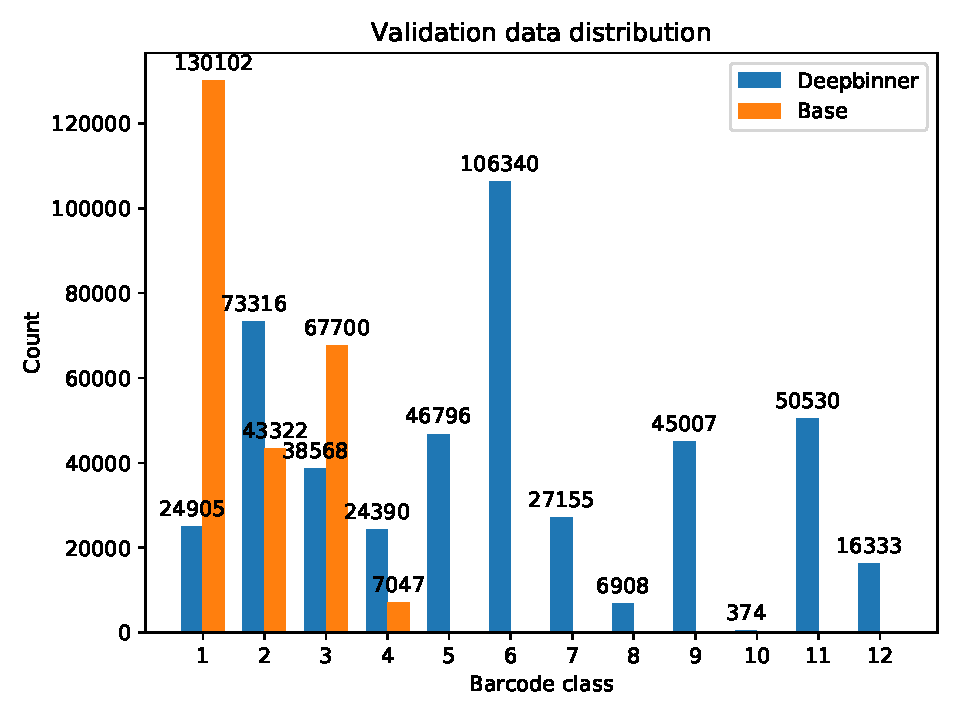
\includegraphics[scale=0.8]{images/dataset_distribution.pdf}
    \caption[Squiggle distributions across both datasets]{Squiggle distribution across the $12$ barcode classes. Note that in both datasets, barcode classes are imbalanced.}
    \label{fig:barcodes_distribution}
\end{figure}


\subsection{Inference of Ground Truth Labels}
The output of Albacore demultiplexing cannot be taken for ground truth for its large error rate ($\approx 10-15\%)$. We will therefore adapt a technique similar to the one presented in Deepbinner article \cite{Deepbinner}. We will align the reads to the reference sequences known for individual organisms used for DNA samples, using the minimap2 software \cite{li2018minimap2}. The output from minimap2 reports for each read the sequence similarity to the best matches, as well as the position of read length aligned to each reference. Out of these alignments, we only keep the reads in which $> 85\%$ of the read length was aligned to exactly one reference sequence.


\section{Datasets Handling}
\label{sec:datasets_handling}
The original representation of reads together with the fact that many reads in fact lack a barcode label, is impractical when it comes to doing experimental work. To get a better grasp on the data needed to train our model, we transformed the training set of squiggles into a more compact format that can be indexed conveniently. For this purpose we created a \texttt{HDF5} file containing $4$ groups, each for one of he first four barcodes from Tab. \ref{tab:training_data_distribution}.


\begin{table}[!ht]
\centering
\begin{tabular}{|l|cccc|}
\hline
Barcode & 1   & 2   & 3   & 4\\
\hline
Count   & 1207 & 647 & 831 & 277\\
\hline
\end{tabular}
\caption{Training dataset distribution.}
\label{tab:training_data_distribution}
\end{table}

For the purpose of our experiments, it would have been convenient to know the exact position of each barcode particular squiggle. However, this information is not contained in the \texttt{fast5} attributes of individual reads directly. Each \texttt{fast5} read file only contains the starting and ending position of the barcode found in its base called sequence. However, we can utilize this information together with the \texttt{events} table to compute the exact positions of the barcodes in the raw signal of the read. The \texttt{events} table is a \texttt{HDF5} dataset that documents the steps of the base calling process. The table starts by creating a \textit{window} $5$-mer from the starting positions of the squiggle and then each line of the table represents the window move of $5$ squiggle values in length. For each such move, an update to the $5$-mer window is made representing the number of bases it moved along (the number is typically between $0$ and $2$). By iterating over the lines of this table and maintaining the number of moves in the base called sequence, we can find the exact starting and ending positions of a barcode in the squiggle. We appended these positions to the attributes of the squiggle in the new \texttt{HDF5} file to be easily accessible at any time. In Fig. \ref{fig:barcode_pos} we see a distribution of the barcode start indices (green), sampled from $200$ squiggles from each of the first $4$ barcodes. The Fig. \ref{fig:barcode_lengts}, displays the distribution of lengths of squiggles corresponding to barcodes, sampled in the same way.

\begin{figure}[!ht]
    \centering
    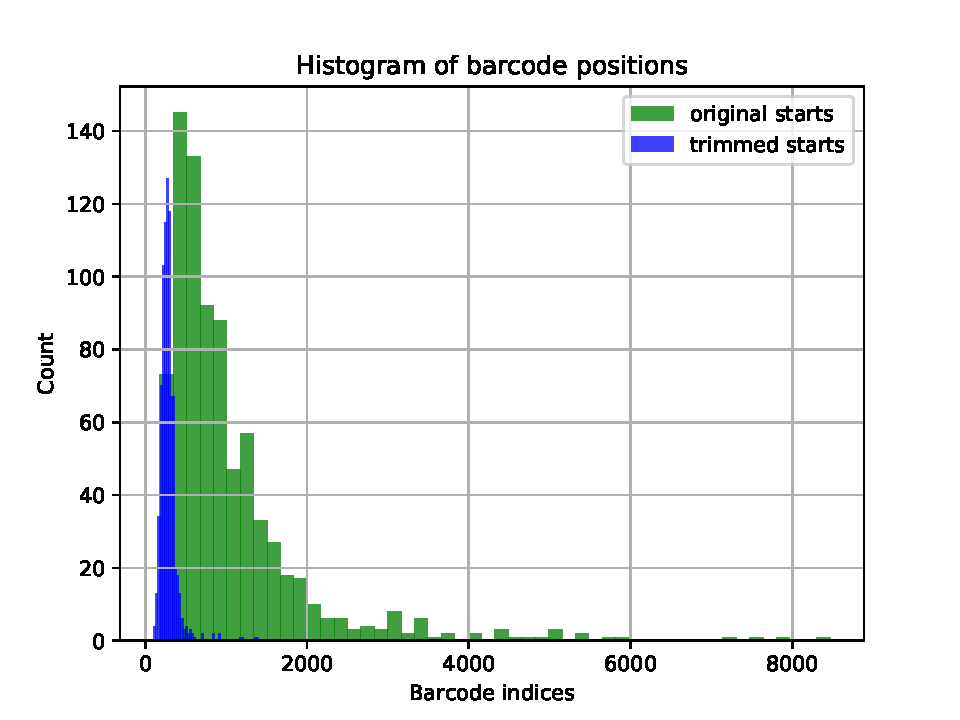
\includegraphics[scale=0.8]{images/trim_hist.pdf}
    \caption[Barcode positions histogram]{The histogram of barcode starting positions in the data (green). We can see that most of the barcodes start after a couple of hundreds of measurements and only a small portion of them after as much as $3000$. The blue histogram stands for the starting positions, after the squiggles were trimmed with our heuristic.}
    \label{fig:barcode_pos}
\end{figure}


\begin{figure}[!ht]
    \centering
    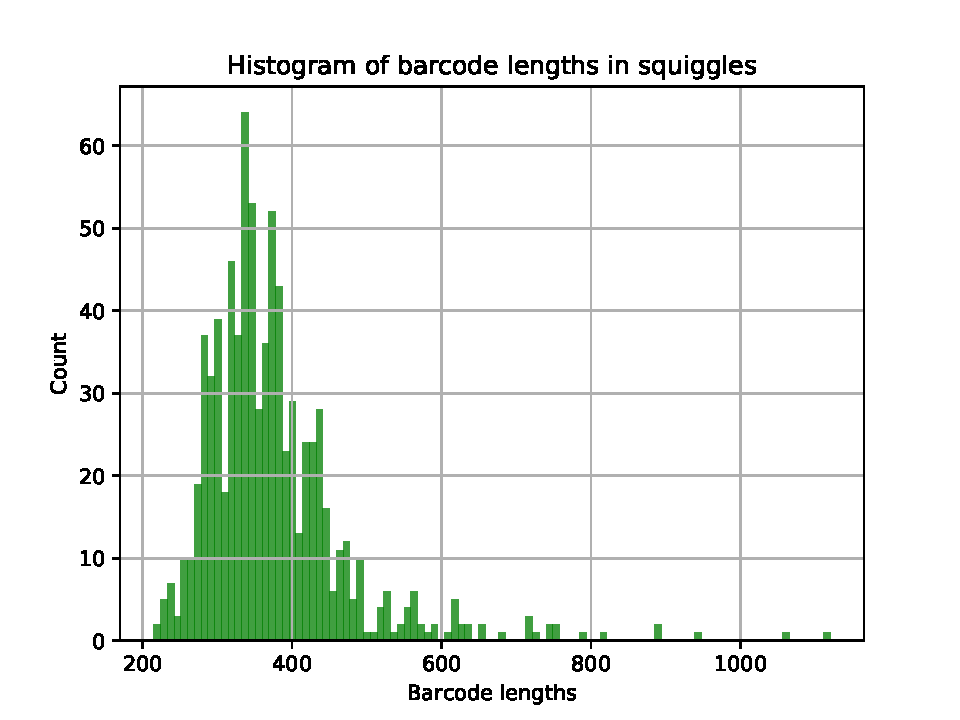
\includegraphics[scale=0.8]{images/barcode_lengths.pdf}
    \caption[Barcode lengths distribution]{The distribution of the lengths of barcodes $1-4$ as they appear in squiggles.}
    \label{fig:barcode_lengts}
\end{figure}


\section{Dealing with Blank Signal Prefixes}
Squiggles produced by nanopore sequencing may possess a \textit{blank} prefix at the beginning, which is corresponding to a random noise. That has been measured in the nanopore between the passage of two DNA strands. This blank signal poses a challenge in two ways. First, the measurement values during such pause are much smaller than in the rest of the squiggle, and hence would produce a very good alignment scores to almost any kind of signal, only due to the fact that the signal values are rather small. Second, such signal further complicates the task of detecting a barcode match by the LDTW similarity, since the blank prefixes vary in length. Moreover, setting a window size that would reliably cover even the longest blank signals would be very time-consuming.

In this light, we devised a simple and fast heuristic that is able to reliably trim the blank signal from almost all of the squiggles. As many squiggles start by the current jumping to very high values and then again dropping back down in the same fashion, we cut off the first $20$ values without an exception. Next, we use the fact that the variance in the blank signal is significantly smaller than in the remainder of the squiggle. We calculate the variance in the second half of the signal within a window of size $W$, and then take the mean of these values as a \textit{variance reference} of non-blank part of the squiggle. This variance reference is progressively compared to the $W$-sized window variances from the start of the signal. This running comparison is terminated when the variance in the windows exceeds the $0.3$ (experimentally estimated constant) multiple of the reference variance. The window size is then halved and the process is repeated from the position where the condition was violated. This is repeated until the window size drops below $5$. The complete process is summarized in a Python code snippet listed below. An example of an output of this heuristic can be seen in Fig. \ref{fig:trimmer_cut}.

\begin{lstlisting}[language=Python, caption={The heuristic for cutting off the blank signal prefixes.}, label={trimmer}]
import numpy as np

    def trim_blank(sig, window=300):
    N = len(sig)
    prefix_size = min(5000, N)
    variances = [np.var(sig[i:i+window]) for i in range(N//2, N-window, window)]
    mean_var = np.mean(variances)
    trim_idx = 20
    while window > 5:
        while np.var(sig[trim_idx: trim_idx + window]) < 0.3*mean_var:
            trim_idx += 1
        window //= 2
    return sig[trim_idx:]
\end{lstlisting}

\begin{figure}[!ht]
    \centering
    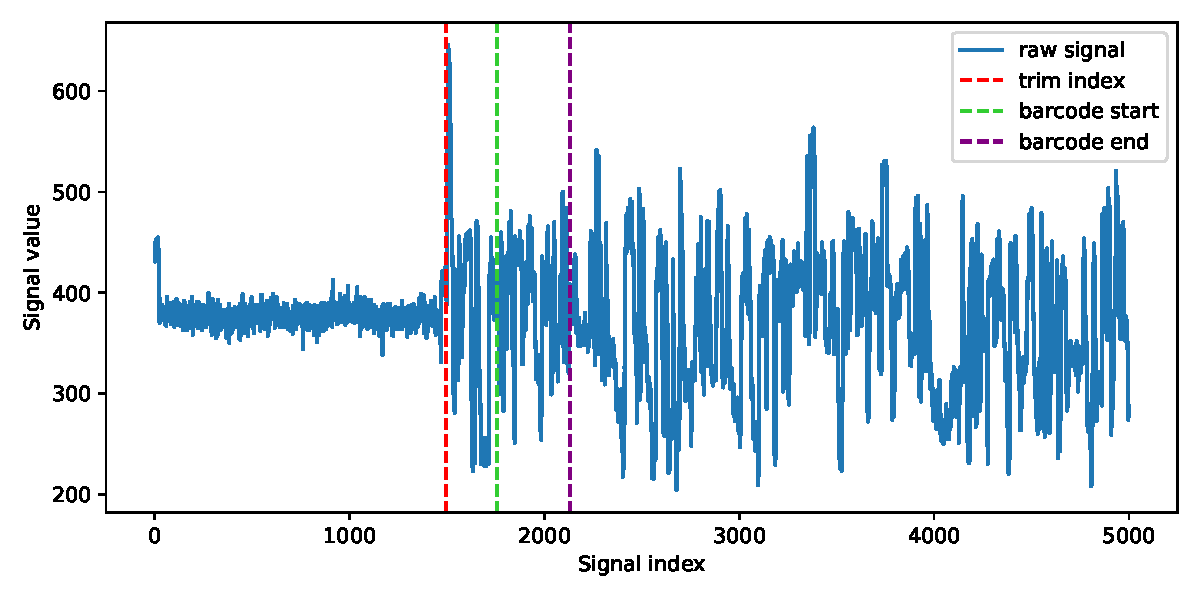
\includegraphics[scale=0.7]{images/trim_1470.pdf}
    \caption[Long blank prefix in a read]{Read with a long blank signal prefix ($\approx 1500$ values). The red line illustrates the index at which our heuristic cuts the signal off, the green and purple lines mark the start and end of the barcode, respectively.}
    \label{fig:trimmer_cut}
\end{figure}

To assess the performance of this heuristic more thoroughly, we tested it on a subsample of our training dataset. For each squiggle, we measured the distance between the position at which our heuristic cuts off the blank signal and the starting position of the barcode sequence begins. The results are summarized in Fig. \ref{fig:trim_errors}. The test was performed on $200$ reads randomly selected from each barcode class from our training dataset. In vast majority of cases, the heuristic trims the squiggles within $500$ signal values of the barcode start position. For the few reads where this did not hold, the blank signal was correctly trimmed, but the barcode signal started later than usual due to the longer signal corresponding to the adapter sequence. There was only a handful of cases where our heuristic did in fact cut a part of the barcode signal. Overall, we can conclude that the heuristic performs satisfactorily.


\begin{figure}[!ht]
    \centering
    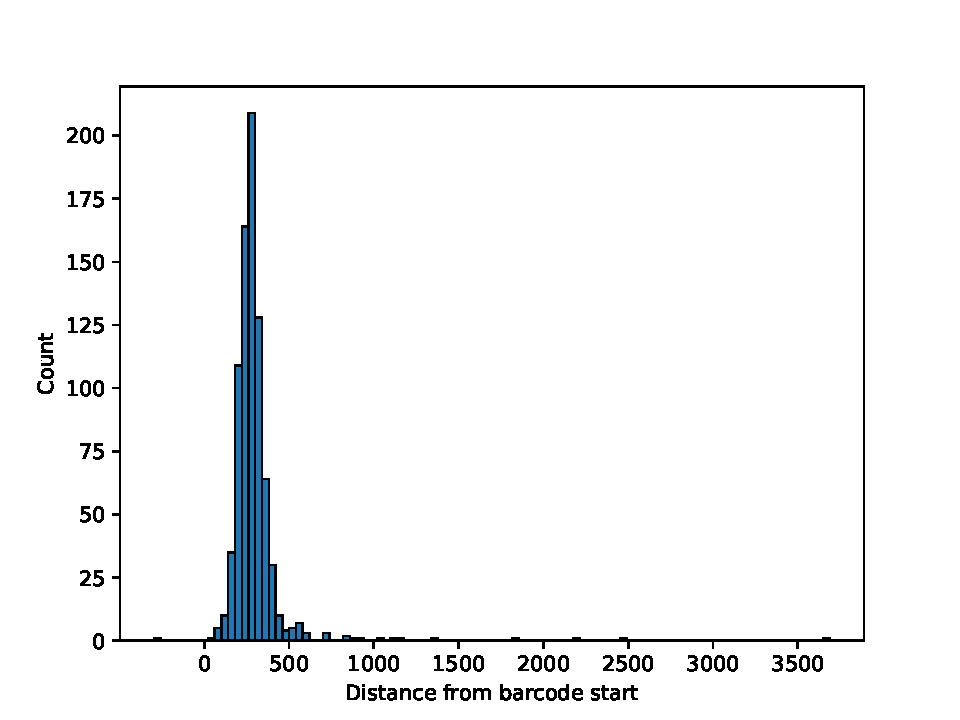
\includegraphics[scale=0.8]{images/trimmer_test.pdf}
    \caption[Histogram of blank prefix trims]{The histogram of distances between the trim index found by our heuristic and the start of the barcode. The small bin in the negative side of the $x$-axis represents cases where our heuristic erroneously cut off a part of of the barcode.}
    \label{fig:trim_errors}
\end{figure}

Fig. \ref{fig:trim_errors} gives us an indicator for selecting the correct prefix window size for our algorithm. If the selected window was too small, we would be analyzing the noise around the adapter sequences instead of barcodes. On the other hand, large windows would lead to computationally intensive analyses. By observing the distribution of barcode lengths as they appear in squiggles in Fig. \ref{fig:barcode_lengts}, we see that the vast majority of the barcodes are under $\approx 500$ values in length. Together with the results form Fig. \ref{fig:trim_errors}, we see a window length of $1000$ as a reasonable choice.

\section{Barcode Signal Modeling}
TO ascertain the similarities between barcodes presented in \ref{tab:barcodes}, we used the $k$-mer model by ONT \cite{KmertablesONT} to simulate a typical signal values produced by as barcdodes pass through the nanopore. For a particular $k$-mer that occurs in the DNA sequence, the $k$-mer model gives the mean value and standard deviation of signal readouts produced as this $k$-mer. W will only consider mean values, which we use to reconstruct the shape of the squiggles corresponding to each barcode. For our model, $k = 6$. The mean squiggle $s_1, s_2, ..., s_{n-5}$ is therefore constructed as

$$s_i = \textsc{kmer-table-mean}[x_ix_{i+1}\cdots x_{i+5}],$$

where $x_1, ..., x_n$ is the nucleotide sequence of the barcode. The resulting values $s_1,...,s_{n-5}$ need to be stretched to resemble a more plausible signal, as there are multiple observations corresponding to each $k$-mer. We achieved this by computing the intermediate values between each pair of subsequent points by a simple linear interpolation \footnote{Linear interpolation: \url{https://en.wikipedia.org/wiki/Linear_interpolation}} such that the lengths of these squiggles are extended to $400$ values. The mean squiggles constructed for the barcodes $1-4$ are showed in Fig. \ref{fig:mean_barcodes}.

\begin{figure}[!ht]
    \centering
    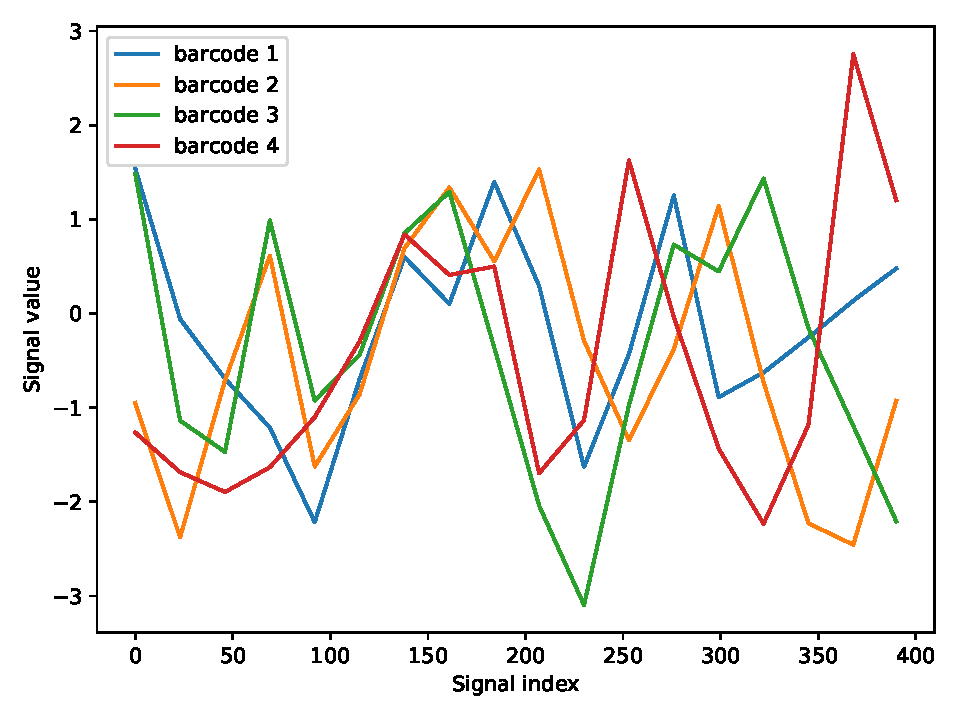
\includegraphics[scale=0.8]{images/barcode_means.pdf}
    \caption[Mean barcode signals]{The squiggles created from the Kmer model table. We can see that the signals are all very similar around the point $150$. Apart from that, barcodes $1$ and $4$ seem to be the most similar among all pairs.}
    \label{fig:mean_barcodes}
\end{figure}

\subsection{Barcode Similarities}
To ascertain how well can we distinguish between these simulated squiggles, we aligned each pair of squiggles with the LDTW and examine the alignment scores as well as the resulting optimal alignment paths. Our LDTW function was able to find considerably good alignments for all pairs of barcodes as can be observed in Fig. \ref{fig:means_collage}. However, we note that our LDTW model was trained on raw, noisy squiggles produced by sequencing and so is not adjusted to this level of smoothness, which is the reason why these alignments are overly optimistic.

\begin{figure}
\centering
\begin{tabular}{cc}
\subfloat{\label{1}}{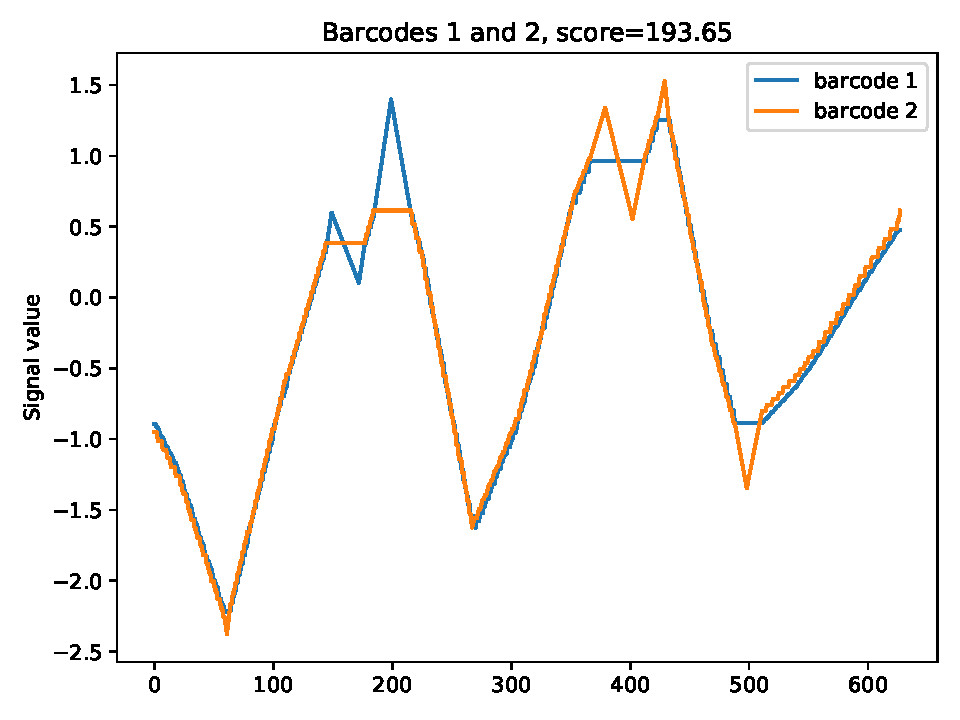
\includegraphics[width = 2.75in]{images/means_comparison/alignment_0_1.pdf}} &
\subfloat{\label{1}}{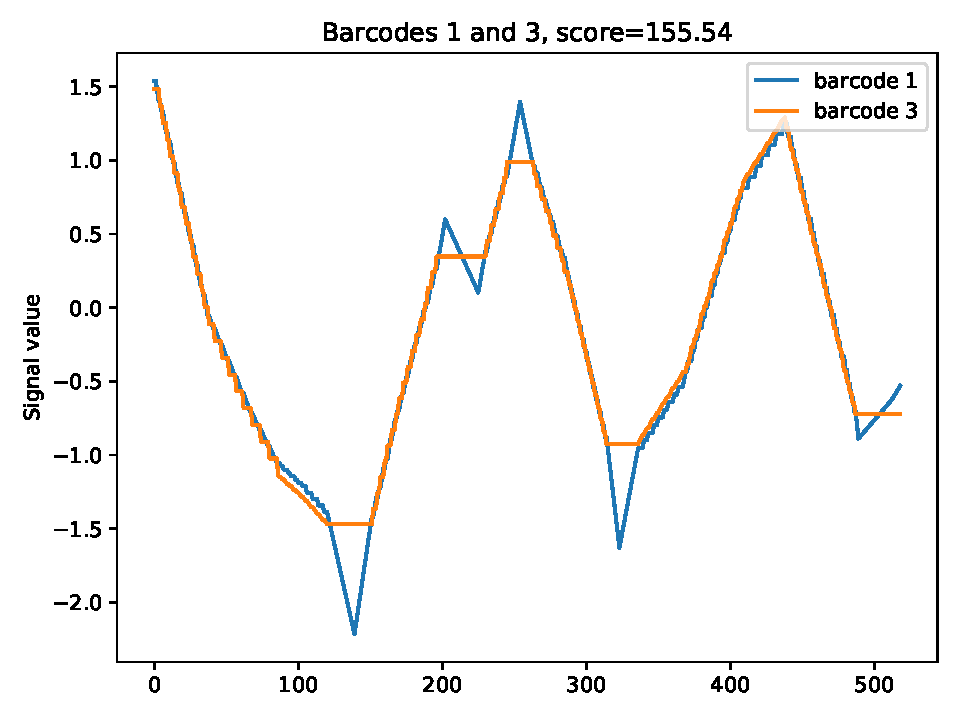
\includegraphics[width = 2.75in]{images/means_comparison/alignment_0_2.pdf}} \\
\subfloat{\label{1}}{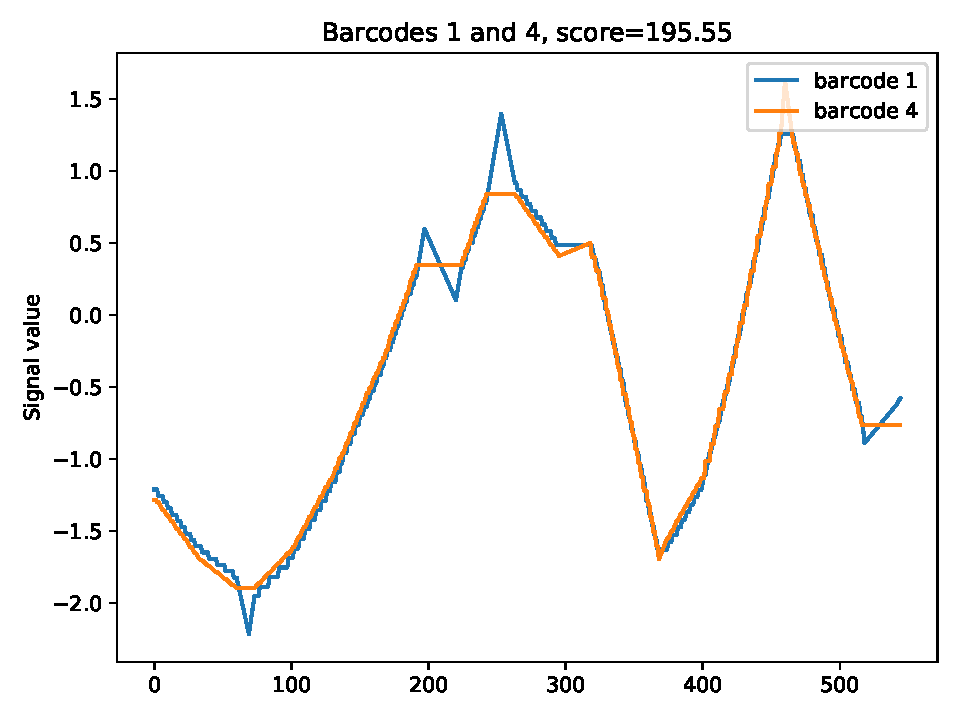
\includegraphics[width = 2.75in]{images/means_comparison/alignment_0_3.pdf}}&
\subfloat{\label{1}}{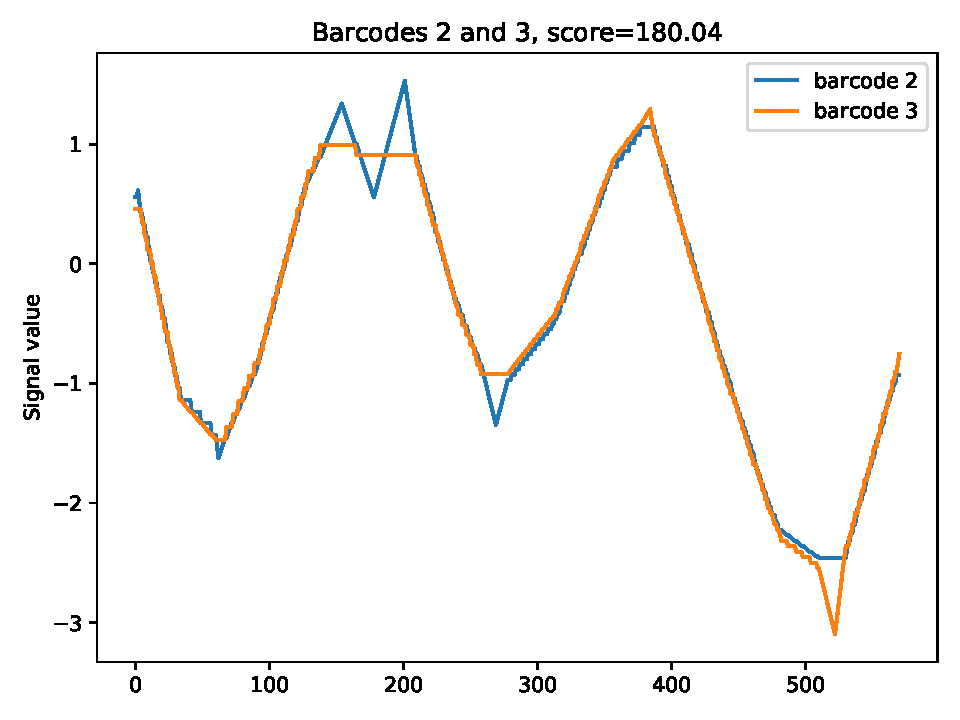
\includegraphics[width = 2.75in]{images/means_comparison/alignment_1_2.pdf}} \\
\subfloat{\label{1}}{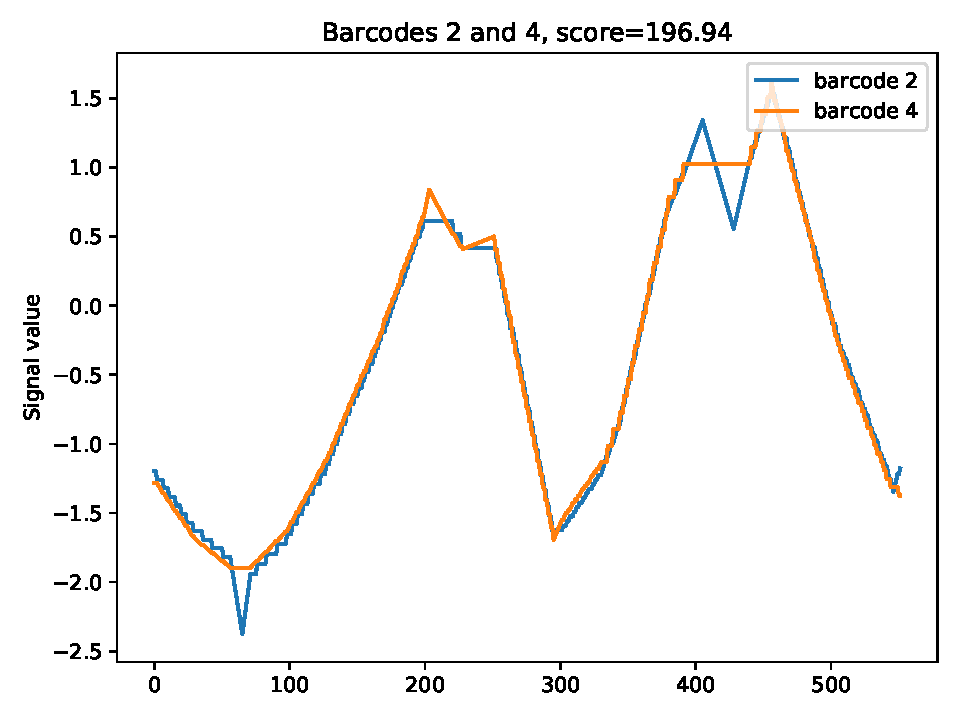
\includegraphics[width = 2.75in]{images/means_comparison/alignment_1_3.pdf}} &
\subfloat{\label{2}}{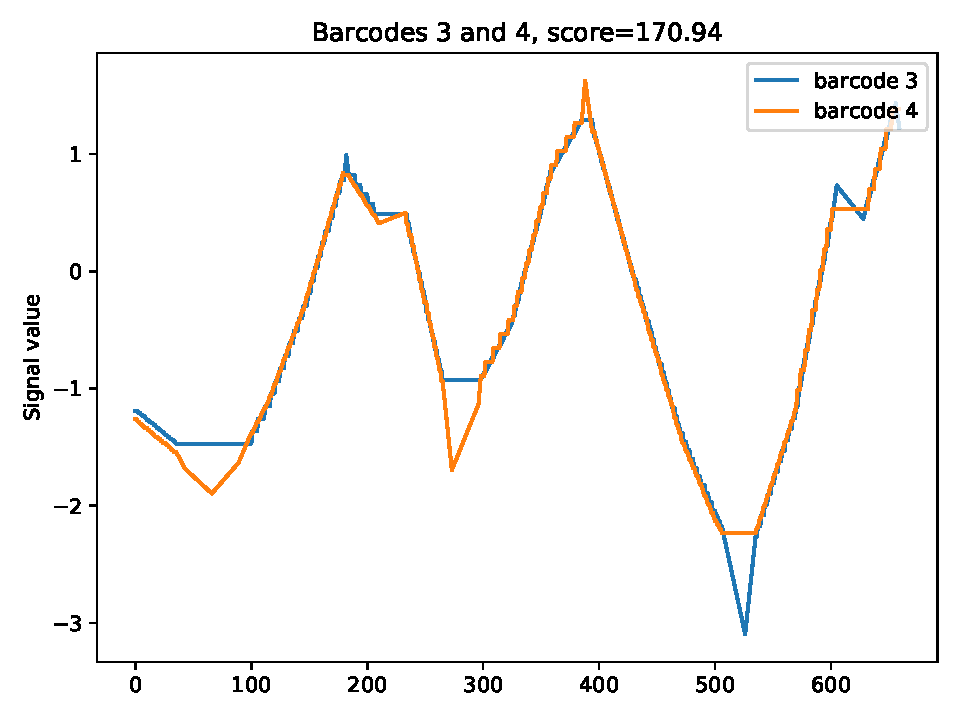
\includegraphics[width = 2.75in]{images/means_comparison/alignment_2_3.pdf}}\\
\end{tabular}
    \caption[LDTW alignments of the mean barcode squiggles]{The LDTW alignments of the simulated squiggles of barcodes $1-4$ of the Native Barcoding Kit. We can see that the squiggles are aligned to each other with a relatively small error, showing occasional departures from their consensus signal.}
    \label{fig:means_collage}
\end{figure}

Let us now examine the inter-barcode similarities in the nucleotide sequences of the barcodes. We applied the Smith-Waterman algorithm (scoring scheme: $\text{match}=1, \text{mismatch}=-1, \text{gap}=-2$) to align all pairs of the first $12$ barcodes of the NBK. The resultning alignment scores are displayed as a heatmap in Fig. \ref{fig:barcodes_SW}. Apparently, some pairs of barcodes are more similar than others, with some pairs achieving the alignment score of $9$ which is a maximum, e.g. barcodes $1$ and $5$. One of the alignments of $1$ and $5$ shown here:

\begin{verbatim}
                            CACAAAGACA-CCGACAAC
                            ****** *** |****|**
                            CACAAA-ACAGACGACTAC
\end{verbatim}
Symbol $*$ marks a match, $|$ a mismatch and $-$ stands for a gap.

However, we are even more interested in how much are these similarities in nucleotide sequences reflected in the raw signal space.

\begin{figure}[!ht]
    \centering
    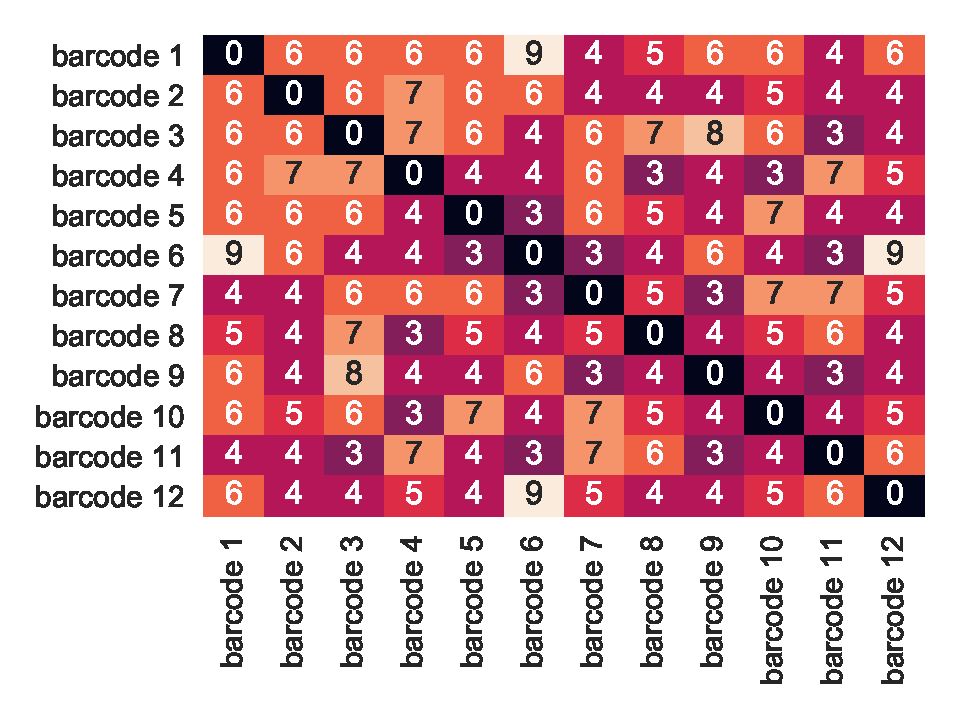
\includegraphics[scale=0.8]{images/SW_12.pdf}
    \caption[Local barcode alignments]{Smith-Waterman alignments of the barcodes $1-12$ of the native barcoding kit. The diagonal is set to $0$ as the trivial case of self-alignment is omitted.}
    \label{fig:barcodes_SW}
\end{figure}

\subsection{Aligning Barcode Models to Signals}
%As we have created a model that represents a notion of an 'average barcode squiggle', a natural question that arises is whether we are able to use it to identify the presence of a barcode in real data by LDTW score. By the construction of the mean barcode squiggles we would expect to find a good match in the average case, however, the smoothness of the mean squiggles may cause problems.

Using the simulated barcode squiggles $M_1, M_2, M_3, M_4$ corresponding to barcodes $1-4$, we generated a balanced sample of $500$ squiggles from each cluster, selected the prefix windows of size $1000$ as we suggested earlier and aligned the mean barcodes to each of them by our LDTW algorithm.

\begin{figure}[!ht]
    \centering
    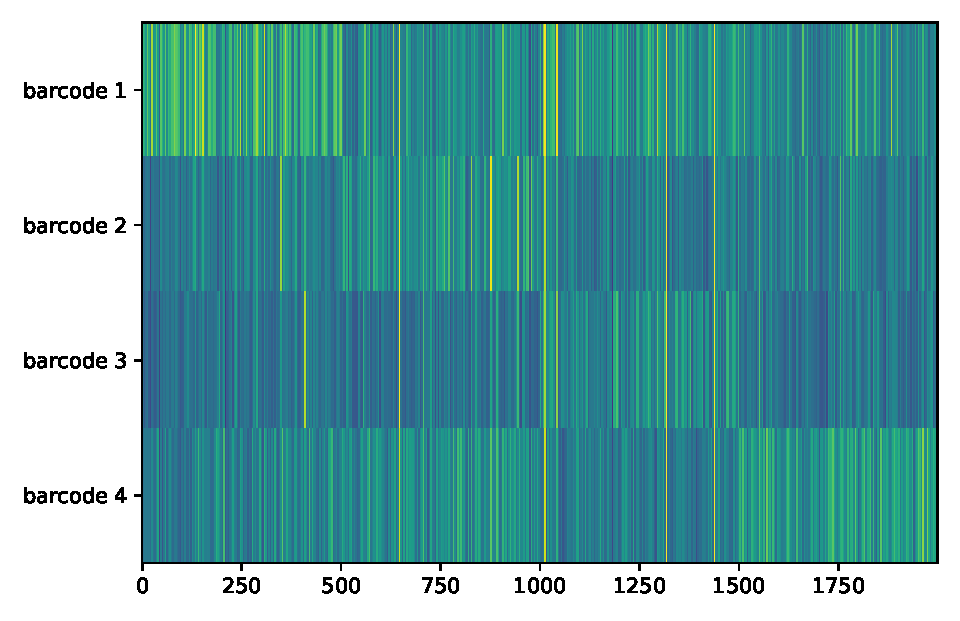
\includegraphics[scale=0.8]{images/align_to_means.pdf}
    \caption[LDTW alignments of mean barcodes to real squiggles]{The LDTW alignments of the simulated squiggles from barcodes $1-4$ from the Native Barcoding Kit to a balanced sample of $2000$ random squiggles ($500$ of each class). Lighter colors represent higher scores. The scores of value $150$ or above were set to $150$ for a clearer visualisation.}
    \label{fig:means_align}
\end{figure}

In Fig. \ref{fig:means_align} we can observe that the scores of the alignments are not always very discriminative. While the barcode $1$ alignes well to squiggles from its own barcode class, there is also a trend of higher scores in to squiggles from the class $2$. The same is true for barcode model $3$ and read samples from class $1$, etc. We can conclude that even tough there are some hints of regions with high/low density, the scores seem to be noisy overall.


\section{Squiggle Normalization}
We will not work with the raw signal values as they come from the sequencing device as they are influenced by the sequencing environment such as voltage changes, noise, etc. We can filter out at least some of the environment effects by unifying the mean and the standard deviation of the squiggles as follows:

\begin{equation}
s_i := \frac{s_i - \mu}{\sigma}
\end{equation}

where $\mu$ is the mean and $\sigma$ is the standard deviation of the squiggle $S$. This is called a z-Score normalization and it is a standard heuristic for preprocessing squiggles \cite{loose2016real}. There are other methods of normalizing squiggles, such as \textit{median normalization} proposed by Stoiber et. al. \cite{Stoiber094672}. We will use the z-score normalization in the rest of our work.

\subsection{Iterative Scaling}
Bo\v{z}a et. al \cite{Boza2017Scaling} introduced iterative scaling method for classical DTW that significantly increased its discriminative power when used in selective sequencing. Their approach was to first perform standard DTW on z-score normalized squiggles $X, Y$ to obtain an alignment path $(u_1, v_1), ...,  (u_k, v_k)$ and subsequently find such parameters $A,B \in \mathbb{R}$ so as to minimize the sum of residuals of aligned squiggles: $\sum_{i=1}^k (Ax_{u_i}  + B - y_{v_i})^2$, which is essentially ordinary least squares problem and can be solved analytically in polynomial time. This process of rescaling can be repeated multiple times for further minimization of the error, though the magnitude of the improvement decreases with each iteration.

This heuristic aims to minimize Euclidean distance of aligned sequences, which is not the same goal as maximal similarity in LDTW. Nevertheless, we tried to use this approach in order to enhance the discriminative power of our LDTW algorithm, with the intention that it could highlight the barcode matches with higher alignment scores. First, aligning the sequences by our LDTW algorithm on z-score normalized sequences. Afterwards, we solved  the linear regression for scaling parameters $A, B$, rescaled the whole length of the prefix window and again run the LDTW algorithm to find a possibly enhanced alignment in case the barcodes match.

We chose $10$ barcodes from classes $1$ and $2$ and performed one set of alignments within class $1$ and the other across both classes.

\begin{figure}[!ht]
    \centering
    \subfloat[Alignments of barcodes $1$ and $1$]
    {{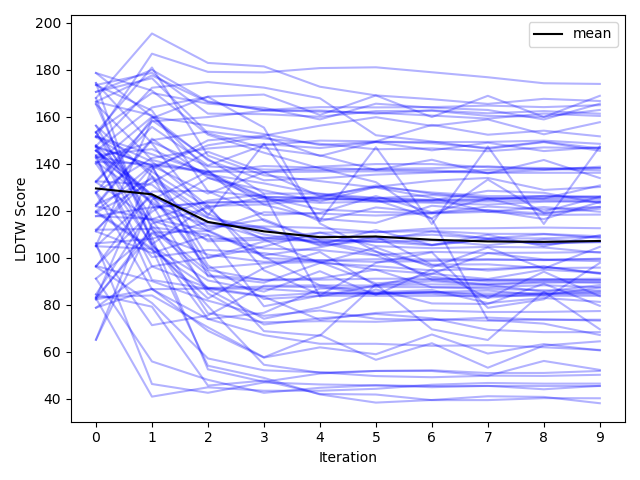
\includegraphics[width=7cm]{images/iterative_scaling_11.png} }}%
    \qquad
    \subfloat[Alignments of barcodes $1$ and $2$]
    {{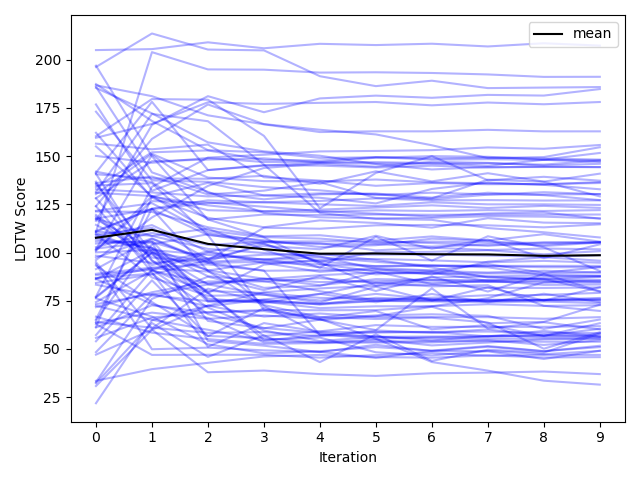
\includegraphics[width=7cm]{images/iterative_scaling_12.png} }}%
    \caption[Iterative scaling]{Nine iteration of the iterative scaling process. The $0$th iteration stands for the initial LDTW score for z-score normalized squiggles.}%
    \label{fig:iterative_scaling}%
\end{figure}

\begin{figure}[ht] % "[t!]" placement specifier just for this example
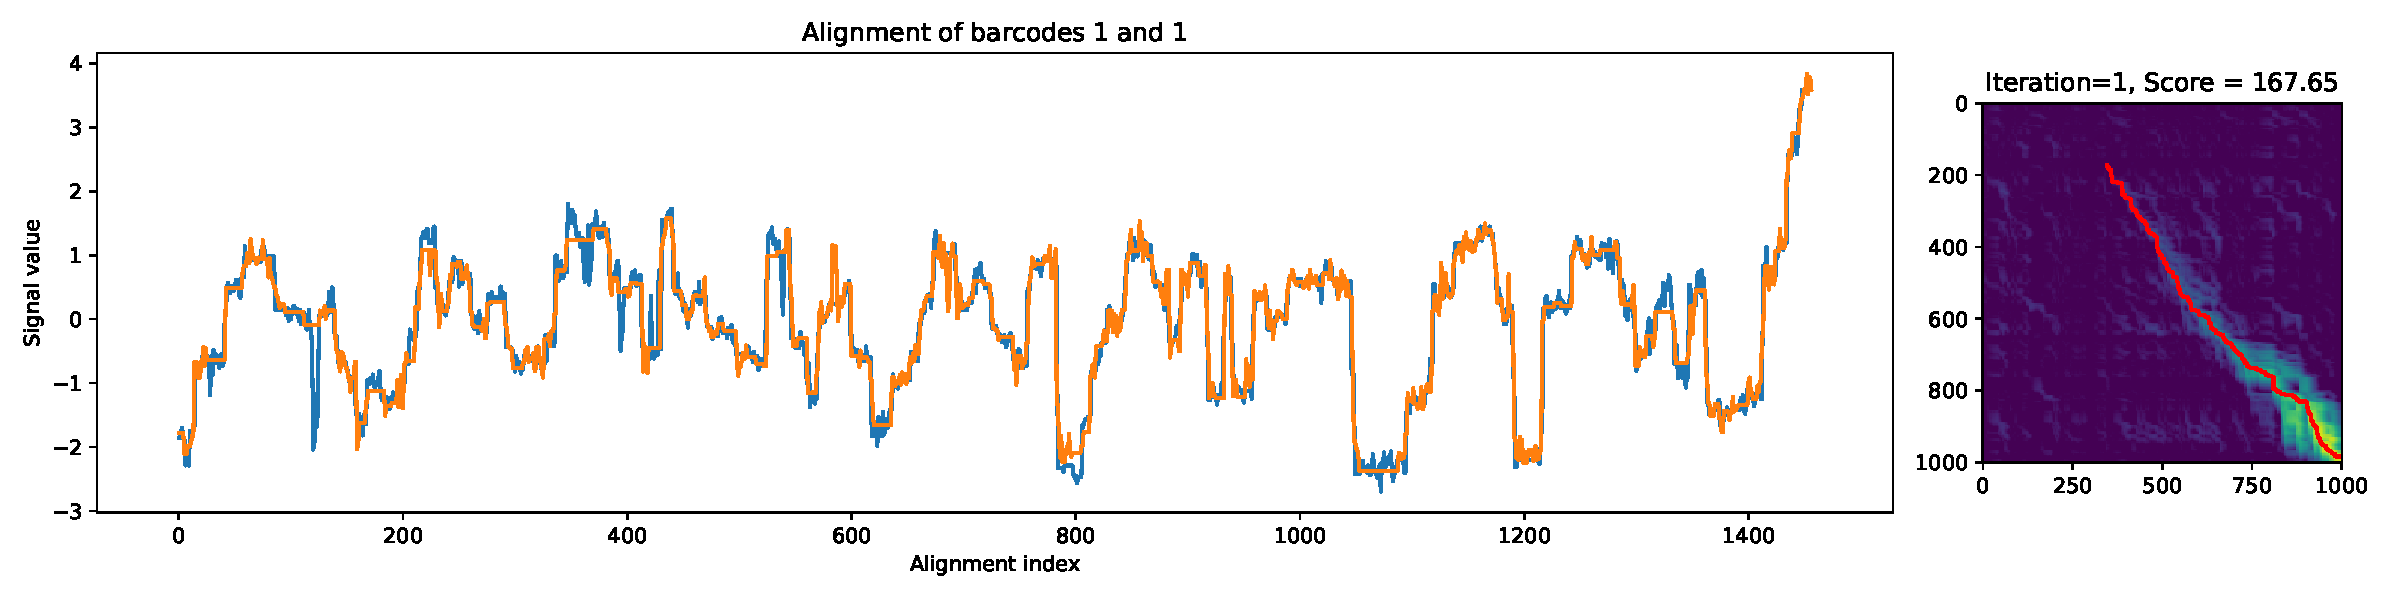
\includegraphics[scale=0.4]{images/scaling/bc1_bc1_1823_1416_it_1.pdf}

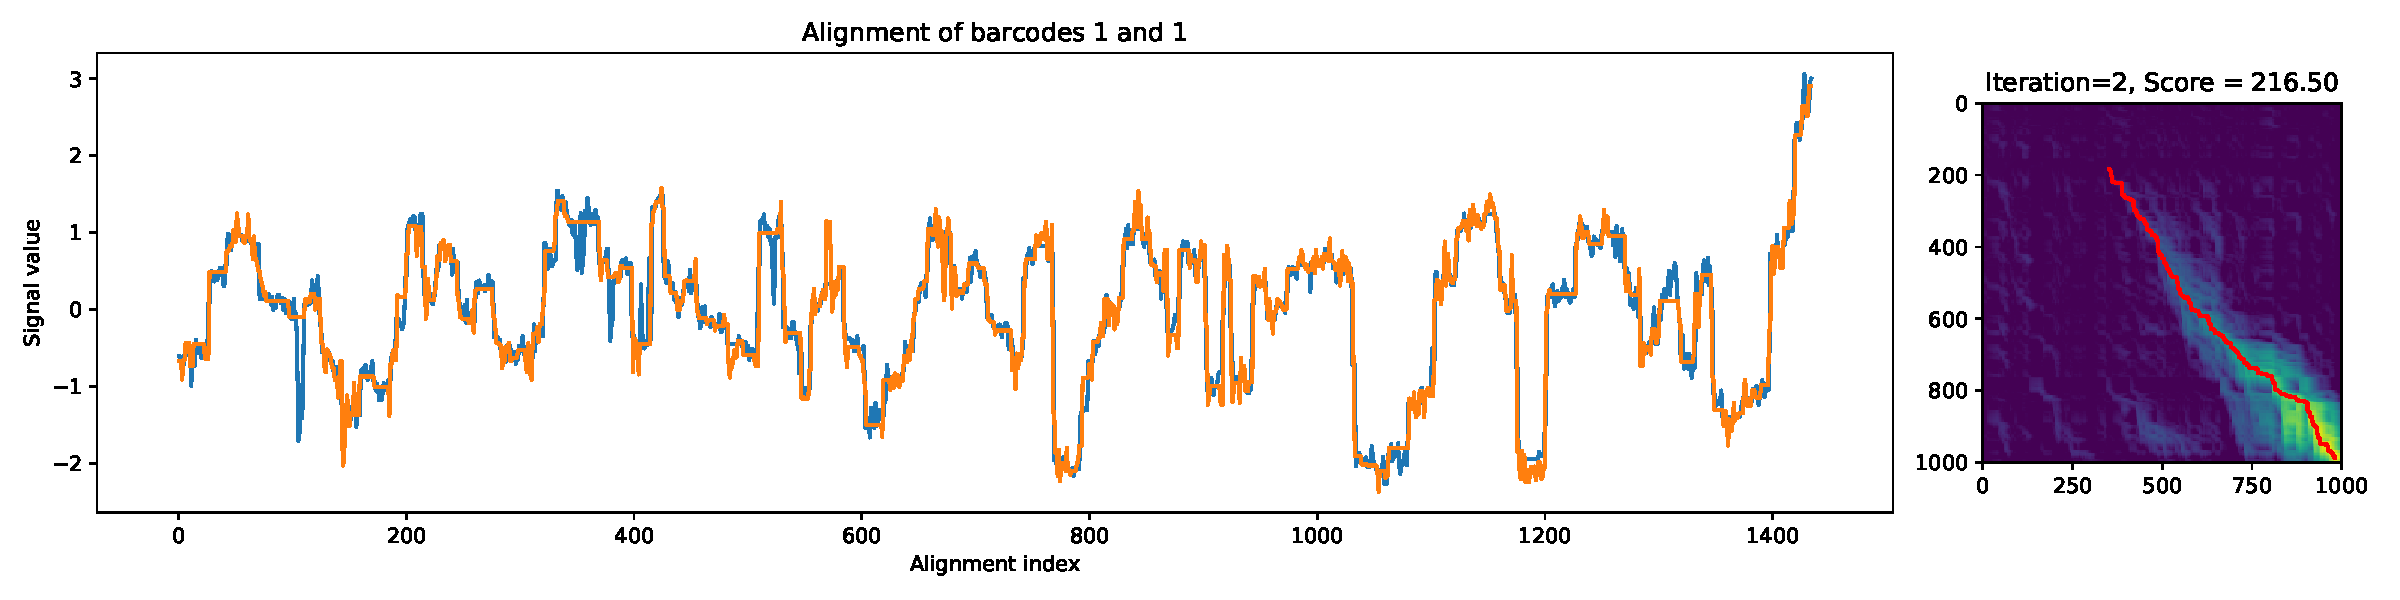
\includegraphics[scale=0.4]{images/scaling/bc1_bc1_1823_1416_it_2.pdf}
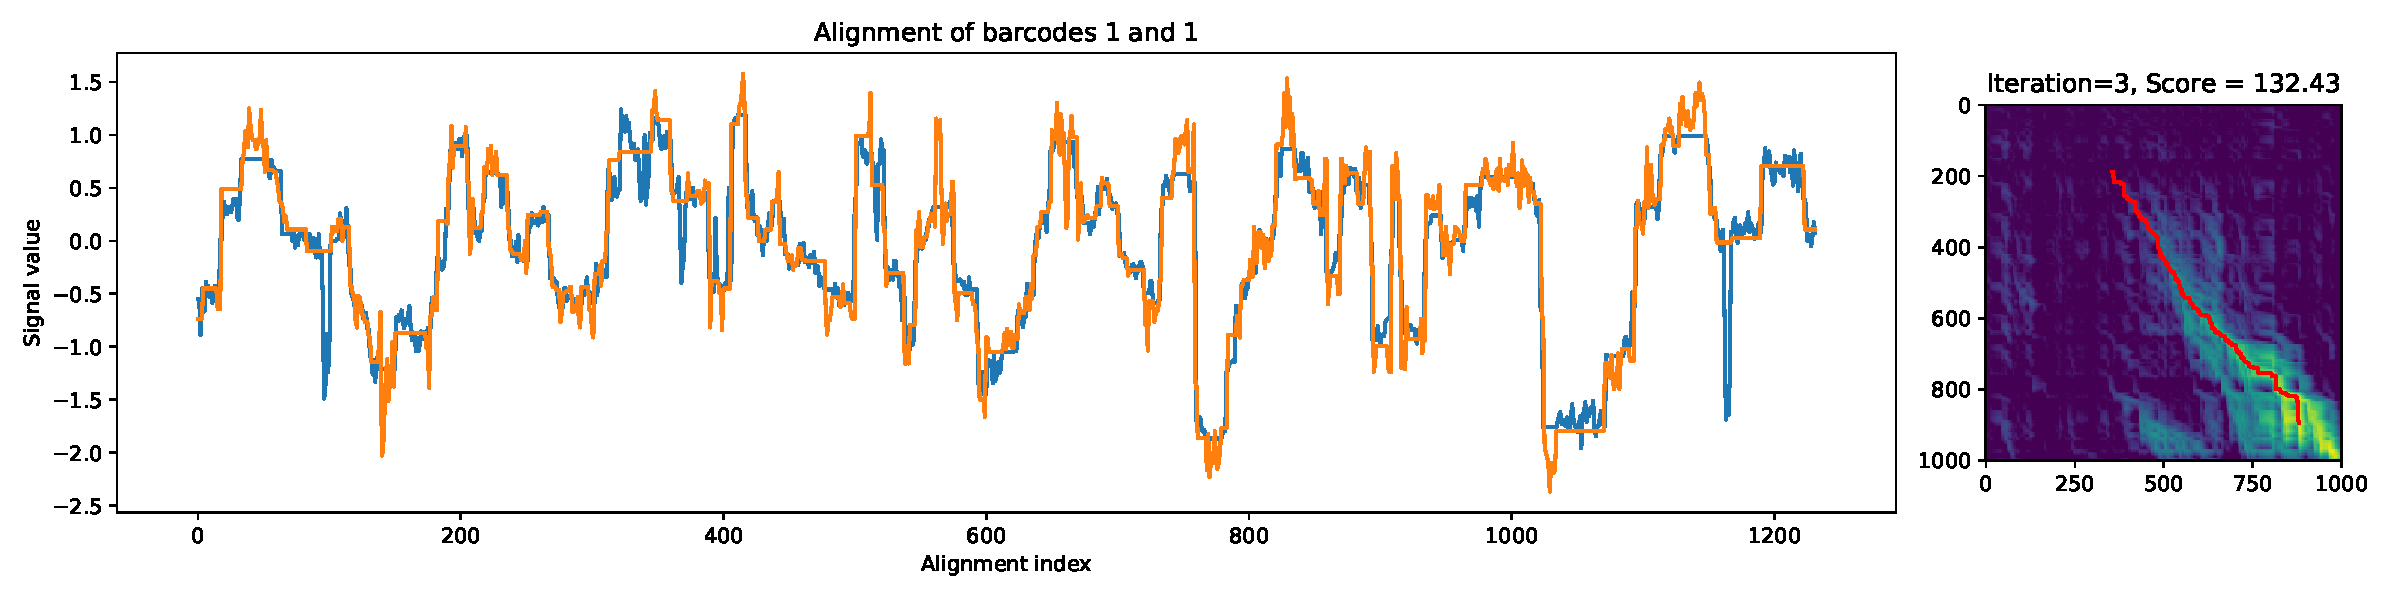
\includegraphics[scale=0.4]{images/scaling/bc1_bc1_1823_1416_it_3.pdf}
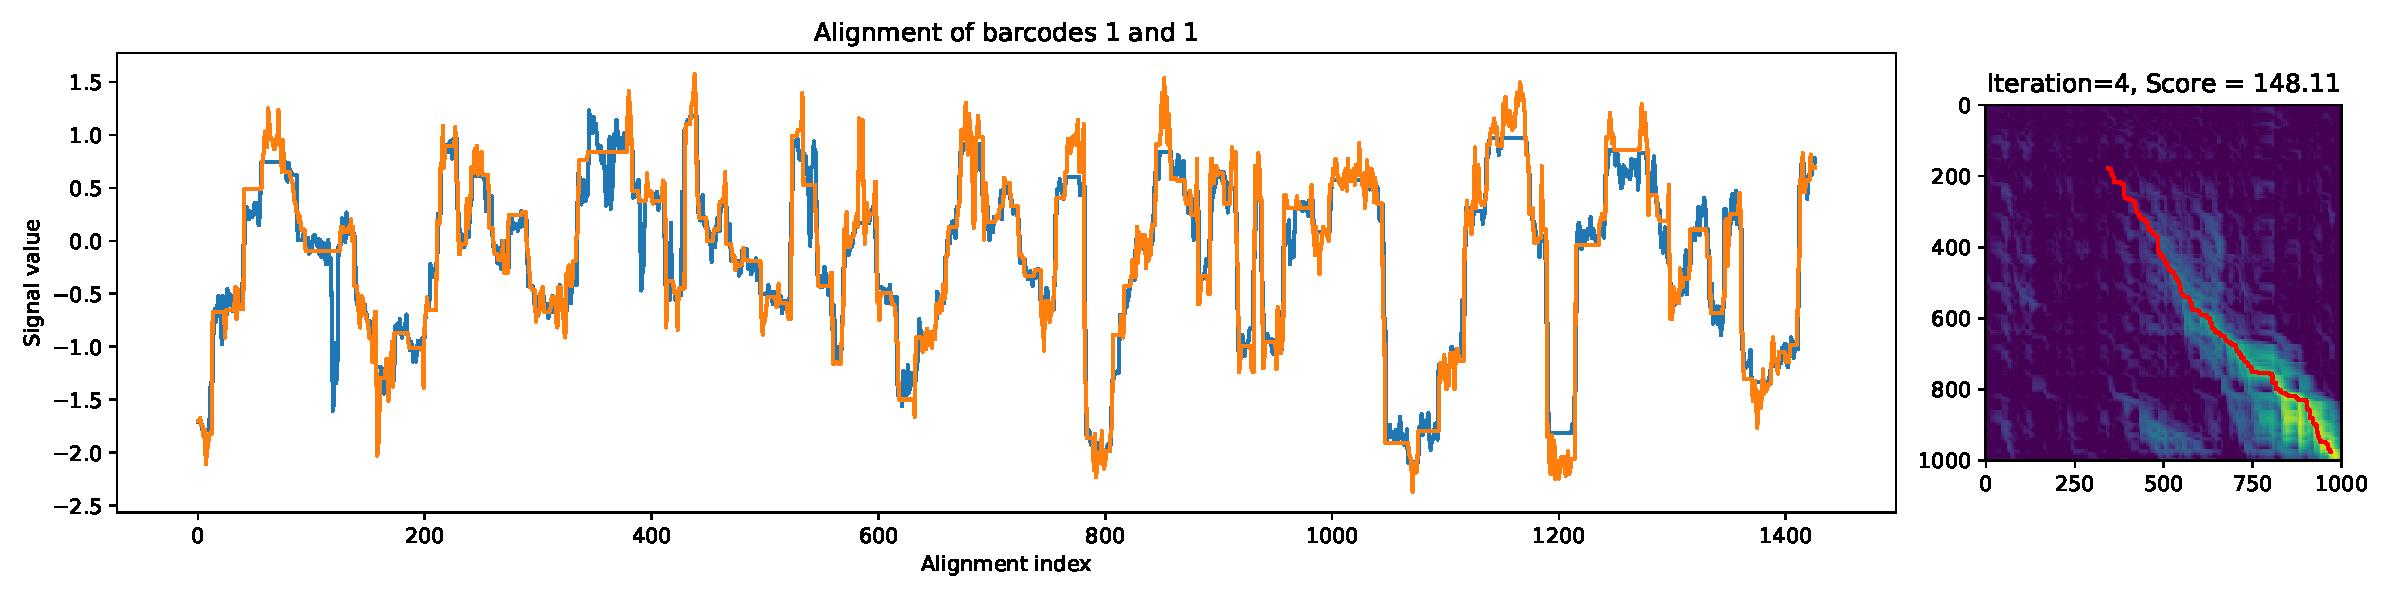
\includegraphics[scale=0.4]{images/scaling/bc1_bc1_1823_1416_it_4.pdf}

\caption[Iterative scaling example]{An example of LDTW alignments during four iterations of the iterative scaling process, using two squiggles from barcode $1$ class.} \label{fig:iterative_scaling_example}
\end{figure}


The results were, however, not satisfactory. In Fig. \ref{fig:iterative_scaling} we can see that there is no improvement in discriminative power. An example of LDTW alignments of two squiggles from barcode $1$ can be seen in Fig. \ref{fig:iterative_scaling_example}.
To use an analogous method in our setting, we would  need to solve the following problem:

\begin{multline}
    \arg\min_{A, B ~\in~ \mathbb{R}} s \left(AX + B, Y \right) =\\
    = \arg\min_{A, B ~\in~ \mathbb{R}} s \left( Ax_{u_1} + B, y_{v_1} \right) ~+~  \cdots ~+~ s \left( Ax_{u_k} + B,  y_{v_k} \right) =\\
    = \arg\min_{A, B ~\in~ \mathbb{R}} f \left( |Ax_{u_1} + B - y_{v_1}| \right) ~+~ \cdots ~+~ f \left( |Ax_{u_k} + B - y_{v_k}| \right)
\end{multline}

where $s$ is our LDTW score function, $f$ is the score function in terms of the distance of two points as in \ref{fig:scoring_scheme} and $(u_1, v_1),...,(u_k, v_k)$ is the alignment path yielded by LDTW. In general it is hard to find any non-trivial assumptions about $f$ and so we would be required to use optimization heuristics of gradient-based algorithms for the minimization (e.g. BFGS \footnote{\url{https://en.wikipedia.org/wiki/Broyden-Fletcher-Goldfarb-Shanno\_algorithm}}) that are mostly very time consuming and do not guarantee the convergence to optimum. Moreover, using such heuristics would make our solution more difficult to interpret, hence we decided not to push towards this direction.
